\documentclass{article}
\usepackage {inputenc, fullpage, amsmath, graphicx, xcolor}

\parindent 0pt

\title{%
   CSc 320: Foundations of Computer Science (Summer 2022)\\
    \Large Alex Holland\\
    Bonus Assignment\\
    }
\date{}

\begin{document}

\maketitle

{\bf Question 1}\\
We want to construct the string-matching automaton for the pattern $P=aabab$ and illustrate its operation on the text string $T=aaababaabaababaab$.\\
First we can compute the transition function $\delta$ table. The states are $\{0,1,2,3,4,5\}$\\
The only accepting state is 5.

\begin{center}
\begin{tabular}{||c c c||} 
 \hline
 State & $a$ & $b$ \\ [0.5ex] 
 \hline\hline
 0 & 1 & 0 \\ 
 \hline
 1 & 2 & 0 \\
 \hline
 2 & 2 & 3 \\
 \hline
 3 & 4 & 0 \\
 \hline
 4 & 2 & 5 \\
 \hline
 5 & 1 & 0 \\
 \hline
\end{tabular}
\end{center}

For the transition table we can construct a state-transition diagram by creating 6 states for the $aabab$ transitions, where state 0 is the start state and state 5 is the only accepting state. 
\begin{center}
    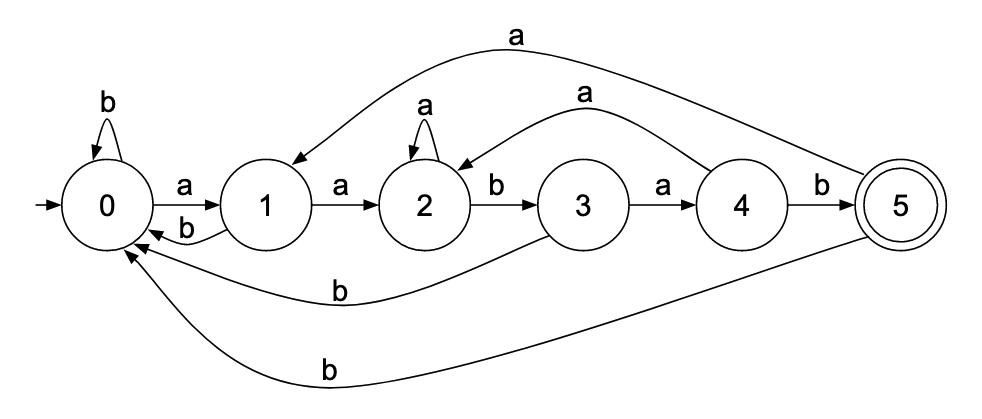
\includegraphics[width=0.75\textwidth]{1.png}
\end{center}

With the state-transition diagram for pattern P created, we now have the ability to apply transition rules to strings that are a subset of the alphabet of the pattern P. Note that only the letters $a$ and $b$ are valid in the string-matching automaton.\\

\break
We can now determine the states of at each index $i$ in the string $T$.

At $i=0$ and $T[0]=\emptyset$ we get: $\delta$ initially in state 0\\
At $i=1$ and $T[1]=a$ we get: $state=\delta(0,a)=1$\\
At $i=2$ and $T[2]=a$ we get: $state=\delta(1,a)=2$\\
At $i=3$ and $T[3]=a$ we get: $state=\delta(2,a)=2$\\
At $i=4$ and $T[4]=b$ we get: $state=\delta(2,b)=3$\\
At $i=5$ and $T[5]=a$ we get: $state=\delta(3,a)=4$\\
At $i=6$ and $T[6]=b$ we get: $state=\delta(4,b)=5$\\
At $i=7$ and $T[7]=a$ we get: $state=\delta(5,a)=1$\\
At $i=8$ and $T[8]=a$ we get: $state=\delta(1,a)=2$\\
At $i=9$ and $T[9]=b$ we get: $state=\delta(2,b)=3$\\
At $i=10$ and $T[10]=a$ we get: $state=\delta(3,a)=4$\\
At $i=11$ and $T[11]=a$ we get: $state=\delta(4,a)=2$\\
At $i=12$ and $T[12]=b$ we get: $state=\delta(2,b)=3$\\
At $i=13$ and $T[13]=a$ we get: $state=\delta(3,a)=4$\\
At $i=14$ and $T[14]=b$ we get: $state=\delta(4,b)=5$\\
At $i=15$ and $T[15]=a$ we get: $state=\delta(5,a)=1$\\
At $i=16$ and $T[16]=a$ we get: $state=\delta(1,a)=2$\\
At $i=17$ and $T[17]=b$ we get: $state=\delta(2,b)=3$\\

Every time we reach state 5 we know we have a match. When matching string $P$ to string $T$ we reached state 5 twice. The shift is the number of positions before the pattern occurrences in the string. We calculate the shift as $shift = i - 5$ at $i = 6$ and $14$:

\begin{equation*} 
\begin{split}
    6 - 5 &= 1\\
    14 - 5 &= 9\\
\end{split}
\end{equation*}

We can summarize our results in the following table, the strings highlighted in $\textcolor{blue}{blue}$ represent strings that match P:
\begin{center}
\begin{tabular}{||c c c||} 
 \hline
 $i$ & $T[i]$ & $\delta$\\ [0.5ex] 
 \hline\hline
 0 & $\emptyset$ & 0 \\ 
 \hline
 1 & $a$ & 1 \\ 
 \hline
 2 & $\textcolor{blue}{a}$ & 2 \\
 \hline
 3 & $\textcolor{blue}{a}$ & 2 \\
 \hline
 4 & $\textcolor{blue}{b}$ & 3 \\
 \hline
  5 & $\textcolor{blue}{a}$ & 4 \\
 \hline
  6 & $\textcolor{blue}{b}$ & 5 \\
 \hline
  7 & $a$ & 1 \\
 \hline
  8 & $a$ & 2 \\
 \hline
  9 & $b$ & 3 \\
 \hline
  10 & $\textcolor{blue}{a}$ & 4 \\
 \hline
  11 & $\textcolor{blue}{a}$ & 2 \\
 \hline
  12 & $\textcolor{blue}{b}$ & 3 \\
 \hline
  13 & $\textcolor{blue}{a}$ & 4 \\
 \hline
  14 & $\textcolor{blue}{b}$ & 5 \\
 \hline
  15 & $a$ & 1 \\
 \hline
  16 & $a$ & 2 \\
 \hline
  17 & $b$ & 3 \\
 \hline
\end{tabular}
\end{center}


\break
{\bf Question 2}\\
We want to compute the prefix function $\pi$ for the pattern $ababbabbabbababbabb$ that we will denote as $P$.\\
The prefix function can be defined as $\pi[q] = max\{k:k<q \; and \; P_k \sqsupset P_q\}$, where $\pi[q]$ is the length of the longest prefix of $P$ that is suffix of $P_q$.\\

The prefix is the left-most end of the pattern. The suffix is the right-most end of the pattern. 
We can determine a list of prefixes and suffixes for the pattern $ababbabbabbababbabb$:\\
The list of prefixes is: $a, ab, aba, abab, ababb, ababba, ababbab, ababbabb, ababbabba, ababbabbab, ababbabbabb, ...$\\
The list of suffixes is: $b, bb, abb, babb, bbabb, abbabb, babbabb, ababbabb, bababbabb, bbababbabb, ...$\\

We want to find the the longest possible suffix of $P$ which is also a the longest possible prefix of $P_q$. This is a subpattern of the string that appears in both the prefix and suffix.\\


For substring of length 1 which is $a$: $\pi[1] = 0$\\
For substring of length 2 which is $ab$: $\pi[2] = 0$\\
For substring of length 3 which is $aba$: $\pi[3] = 1$, because it starts and ends with $a$\\
For substring of length 4 which is $abab$: $\pi[4] = 2$, because it starts and ends with $ab$\\
For substring of length 5 which is $ababb$: $\pi[5] = 0$, because it starts with $a$ and ends with $b$\\
For substring of length 6 which is $ababba$: $\pi[6] = 1$, because it starts and ends with $a$\\
For substring of length 7 which is $ababbab$: $\pi[7] = 2$, because it starts and ends with $ab$\\
For substring of length 7 which is $ababbabb$: $\pi[8] = 0$, because it starts with $a$ and ends with $b$\\
For substring of length 7 which is $ababbabba$: $\pi[9] = 1$, because it starts and ends with $a$\\
For substring of length 7 which is $ababbabbab$: $\pi[10] = 2$, because it starts and ends with $ab$\\
For substring of length 7 which is $ababbabbabb$: $\pi[11] = 0$, because it starts with $a$ and ends with $b$\\
For substring of length 7 which is $ababbabbabba$: $\pi[12] = 1$, because it starts and ends with $a$\\
For substring of length 7 which is $ababbabbabbab$: $\pi[13] = 2$, because it starts and ends with $ab$\\
For substring of length 7 which is $ababbabbabbaba$: $\pi[14] = 3$, because it starts and ends with $aba$\\
For substring of length 7 which is $ababbabbabbabab$: $\pi[15] = 4$, because it starts and ends with $abab$\\
For substring of length 7 which is $ababbabbabbababb$: $\pi[16] = 5$, because it starts and ends with $ababb$\\
For substring of length 7 which is $ababbabbabbababba$: $\pi[17] = 6$, because it starts and ends with $ababba$\\
For substring of length 7 which is $ababbabbabbababbab$: $\pi[18] = 7$, because it starts and ends with $ababbab$\\
For substring of length 7 which is $ababbabbabbababbabb$: $\pi[19] = 8$, because it starts and ends with $ababbabb$\\

Here we can see that that the longest possible suffix is $ababbabb$ as it appears in both the left-most and right-most part of the pattern $P$.\\

The results of the above calculations can be shown in the table of values $\pi$ for the pattern $P$:
\begin{center}
\begin{tabular}{||c c c||} 
 \hline
 $i$ & $P[i]$ & $\pi[i]$\\ [0.5ex] 
 \hline\hline
 1 & $a$ & 0 \\ 
 \hline
 2 & $b$ & 0 \\
 \hline
 3 & $a$ & 1 \\
 \hline
 4 & $b$ & 2 \\
 \hline
  5 & $b$ & 0 \\
 \hline
  6 & $a$ & 1 \\
 \hline
  7 & $b$ & 2 \\
 \hline
  8 & $b$ & 0 \\
 \hline
  9 & $a$ & 1 \\
 \hline
  10 & $b$ & 2 \\
 \hline
  11 & $b$ & 0 \\
 \hline
  12 & $a$ & 1 \\
 \hline
  13 & $b$ & 2 \\
 \hline
  14 & $a$ & 3 \\
 \hline
  15 & $b$ & 4 \\
 \hline
  16 & $b$ & 5 \\
 \hline
  17 & $a$ & 6 \\
 \hline
  18 & $b$ & 7 \\
 \hline
  19 & $b$ & 8 \\
  \hline
\end{tabular}
\end{center}


The prefix function $\pi$ can be determined by scanning substrings of $P$ of size $q$ from left-to-right starting from an index $i=1$ and determining if the prefix is the same as the suffix. For example, a substring of $P$ of length 4 which would be $abab$, $ab$ appears at both the start and end of the substring so by the prefix function $\pi[q] = max\{k:k<q \; and \; P_k \sqsupset P_q\}$ we can determine that $\pi[4] = 2$. We continue this process for all indexes of $P$ (from $i=1$ to $i=19$).


\end{document}
